\chapter{Initial Verification of Quillen Models} \label{chap:app-quillen-rework}

Many finite element analysis software packages support the use of input files with a proprietary keyword syntax.
Examples of this syntax include APDL (ANSYS parametric design language) and keyword syntax in Abaqus.
Creating models with this method is more difficult for new users than with the graphical interactive method.
However, since the keyword method is much closer to writing programs in a high-level programming language, it is much easier to isolate differences between models based off the differences in their input files.
See \Cref{fig:material-apdl} for an example of a material property definition in APDL syntax, and \Cref{fig:material-abaqus-keyword} for the same material property definition in Abaqus keyword syntax.
In both examples, the elastic modulus \(E\)\nomenclature[1E]{\(E\)}{elastic modulus} is defined on the first line, Poisson's ratio \(\nu\)\nomenclature[2\nu]{\(\nu\)}{Poisson's ratio} is defined on the second line, and both can be referenced wherever needed afterwards.

\begin{figure}[bp]
\begin{lstlisting}[language={APDL}]
! Define parameters
E=30.0e6
NU=0.3
! Set material properties
MP,EX,1,E
MP,PRXY,1,NU
\end{lstlisting}
\caption{Material definition in APDL syntax \label{fig:material-apdl}}
\end{figure}
\begin{figure}[bp]
\begin{lstlisting}[language={Abaqus}]
** Define parameters
*PARAMETER
E=30.0e6
NU=0.3
** Set material properties
*MATERIAL, NAME=STEEL
*ELASTIC
<E>, <NU>
\end{lstlisting}
\caption{Material definition in Abaqus keyword syntax \label{fig:material-abaqus-keyword}}
\end{figure}

One disadvantage to the APDL and Abaqus keyword languages is that both store all parameters in a single global scope.
That is, they require any variable (for example, \verb|NU|) to have the same meaning at all places in the code, making it more difficult to describe a problem involving both Poisson's ratio (\( \nu \) in solid mechanics) and kinematic viscosity (\( \nu \) in fluid mechanics).
Even if the variables were renamed to have distinct names (for example, \verb|PR| and \verb|KV|), the code would still require everyone using the set of code to agree on one set of names, making code sharing throughout a research community more difficult.

Abaqus has supported a second input syntax since at least version 6.2---writing models in Python.
Python is a dynamic general-purpose language used for a variety of different applications.
It allows for the creation of functions and modules for code reuse, and supports user-defined data structures to pass data around a program.
An example of a material property definition in Abaqus Python scripting syntax is shown in \Cref{fig:material-abaqus-python}.
\begin{figure}[bp]
\begin{lstlisting}
def setMaterial(model, E=200e9, nu=0.3): # a function
    model.Material(name='Steel')
    model.materials['Steel'].Elastic(table=((E, nu), ))
    # function ends here, main program follows

elasticModulus=30e6 # define parameters
PoissonRatio=0.3
# call functions to create model, set material
myModel = createModel(modelName='McClung-1')
setMaterial(E=elasticModulus,
            nu=PoissonRatio,
            model=myModel)
\end{lstlisting}
\caption{Material definition in Abaqus Python syntax \label{fig:material-abaqus-python}}
\end{figure}

Though the Python version of the material property definition is more verbose than either of the keyword versions of the definition, it is arguably more readable to an infrequent user.
The code also demonstrates four valuable features of Python scripting: the ability to create user-defined functions, the existence of a local variable scope for functions (so that parameters are not defined in a global scope by default), the ability to pass named parameters to functions in any order, and the ability to have default values for any parameters not defined in the function call.
The existence of functions is critical for a program to be easily maintained: if an error is found in a function, it can be corrected once, and that correction automatically propagates everywhere the function was used.
If an error is found in an equation that has been copied and pasted repeatedly (due to a lack of functions in the language), the error must be corrected everywhere the equation exists.

Local parameter scopes are very helpful: they remove the requirement that a variable name have one and only one meaning throughout a body of code, and throughout any code that will ever be used with it.
Default values for parameters and the ability to use named parameters in any order are convenient.
Both of these features enable a research community to coordinate on what set of parameters needs to be passed to a function, and what result that function returns, but places no restrictions on what the parameters or result should be named.
This allows the research community to be more loosely coordinated, and for them to share code more easily with fewer modifications.

Working from a basic Python program for elliptical surface cracks given in the Abaqus~6.11-1 Benchmarks Manual \citeyearpar{abaqus-611-benchmarks-manual}, a new program has been developed to reliably and repeatably analyze surface cracks in plates for any valid combination of plate geometry, crack geometry, material properties, and remote pressures.
This program includes functions for:
\begin{itemize}
\item creation of plate geometry,
\item creation of an elliptical path representing the crack front,
\item sweeping two circular profiles along the elliptical path to create regions for singularity elements and transitional elements near the crack front,
\item assembling the plate and swept profiles into a single assembly,
\item partitioning the plate to enable focused hexahedral meshing throughout the plate,
\item assignment of simple elastic or Ramberg-Osgood elastic-plastic material properties,
\item creation of geometry sets for the traction surface, symmetry planes, and crack front,
\item definition of contour integral \J along the crack front,
\item assignment of mesh sizes (both default and exceptions along specific edges,
\item meshing the model regions with singularity elements, transitional elements, or regular hexahedral elements,
\item creation of load step and boundary conditions,
\item creation of history output requests to track values along the crack front as appropriate (\J for elastic-plastic models; \J, \K and tangential stress for elastic models),
\item creation of job input file,
\item submission of input file for analysis,
\item reading \J values from the resulting Abaqus output database (ODB)\nomenclature[1O]{ODB}{Abaqus output database},
\item converting the \J values into \hone values analogous to those in \Cref{eq:h1mcclung}, and
\item writing \hone values and crack node coordinates to a text file.
\end{itemize}

The complete program contains approximately 1250 lines of Python code and comments (a total of \SI{66}{\kilo\byte} of disk space), with 1100 lines separated into reusable modules or libraries that can be used for any semi-elliptical crack model.
By comparison, a small input file (approximately \num{2300} elements and \num{11000} nodes) may contain over \num{17000} lines and over \SI{1}{\mega\byte} of disk space.
Any model and its corresponding Abaqus input file can be generated within \SI{10}{\second} on an Intel Core2 Duo laptop, enabling quick generation of a set of models to be solved on a high-performance compute cluster or the laptop itself as needed.
Examples of two of the new models are shown in \Crefrange{fig:model1-assembly}{fig:model9-assembly}.
The text file containing node numbers, coordinates, and \hone values can be imported into MATLAB, and graphs can be created.
The additional automation reduces opportunities for random errors in copying and pasting results, inconsistent parameter changes, and related issues.

  \begin{figure}
    \centering
    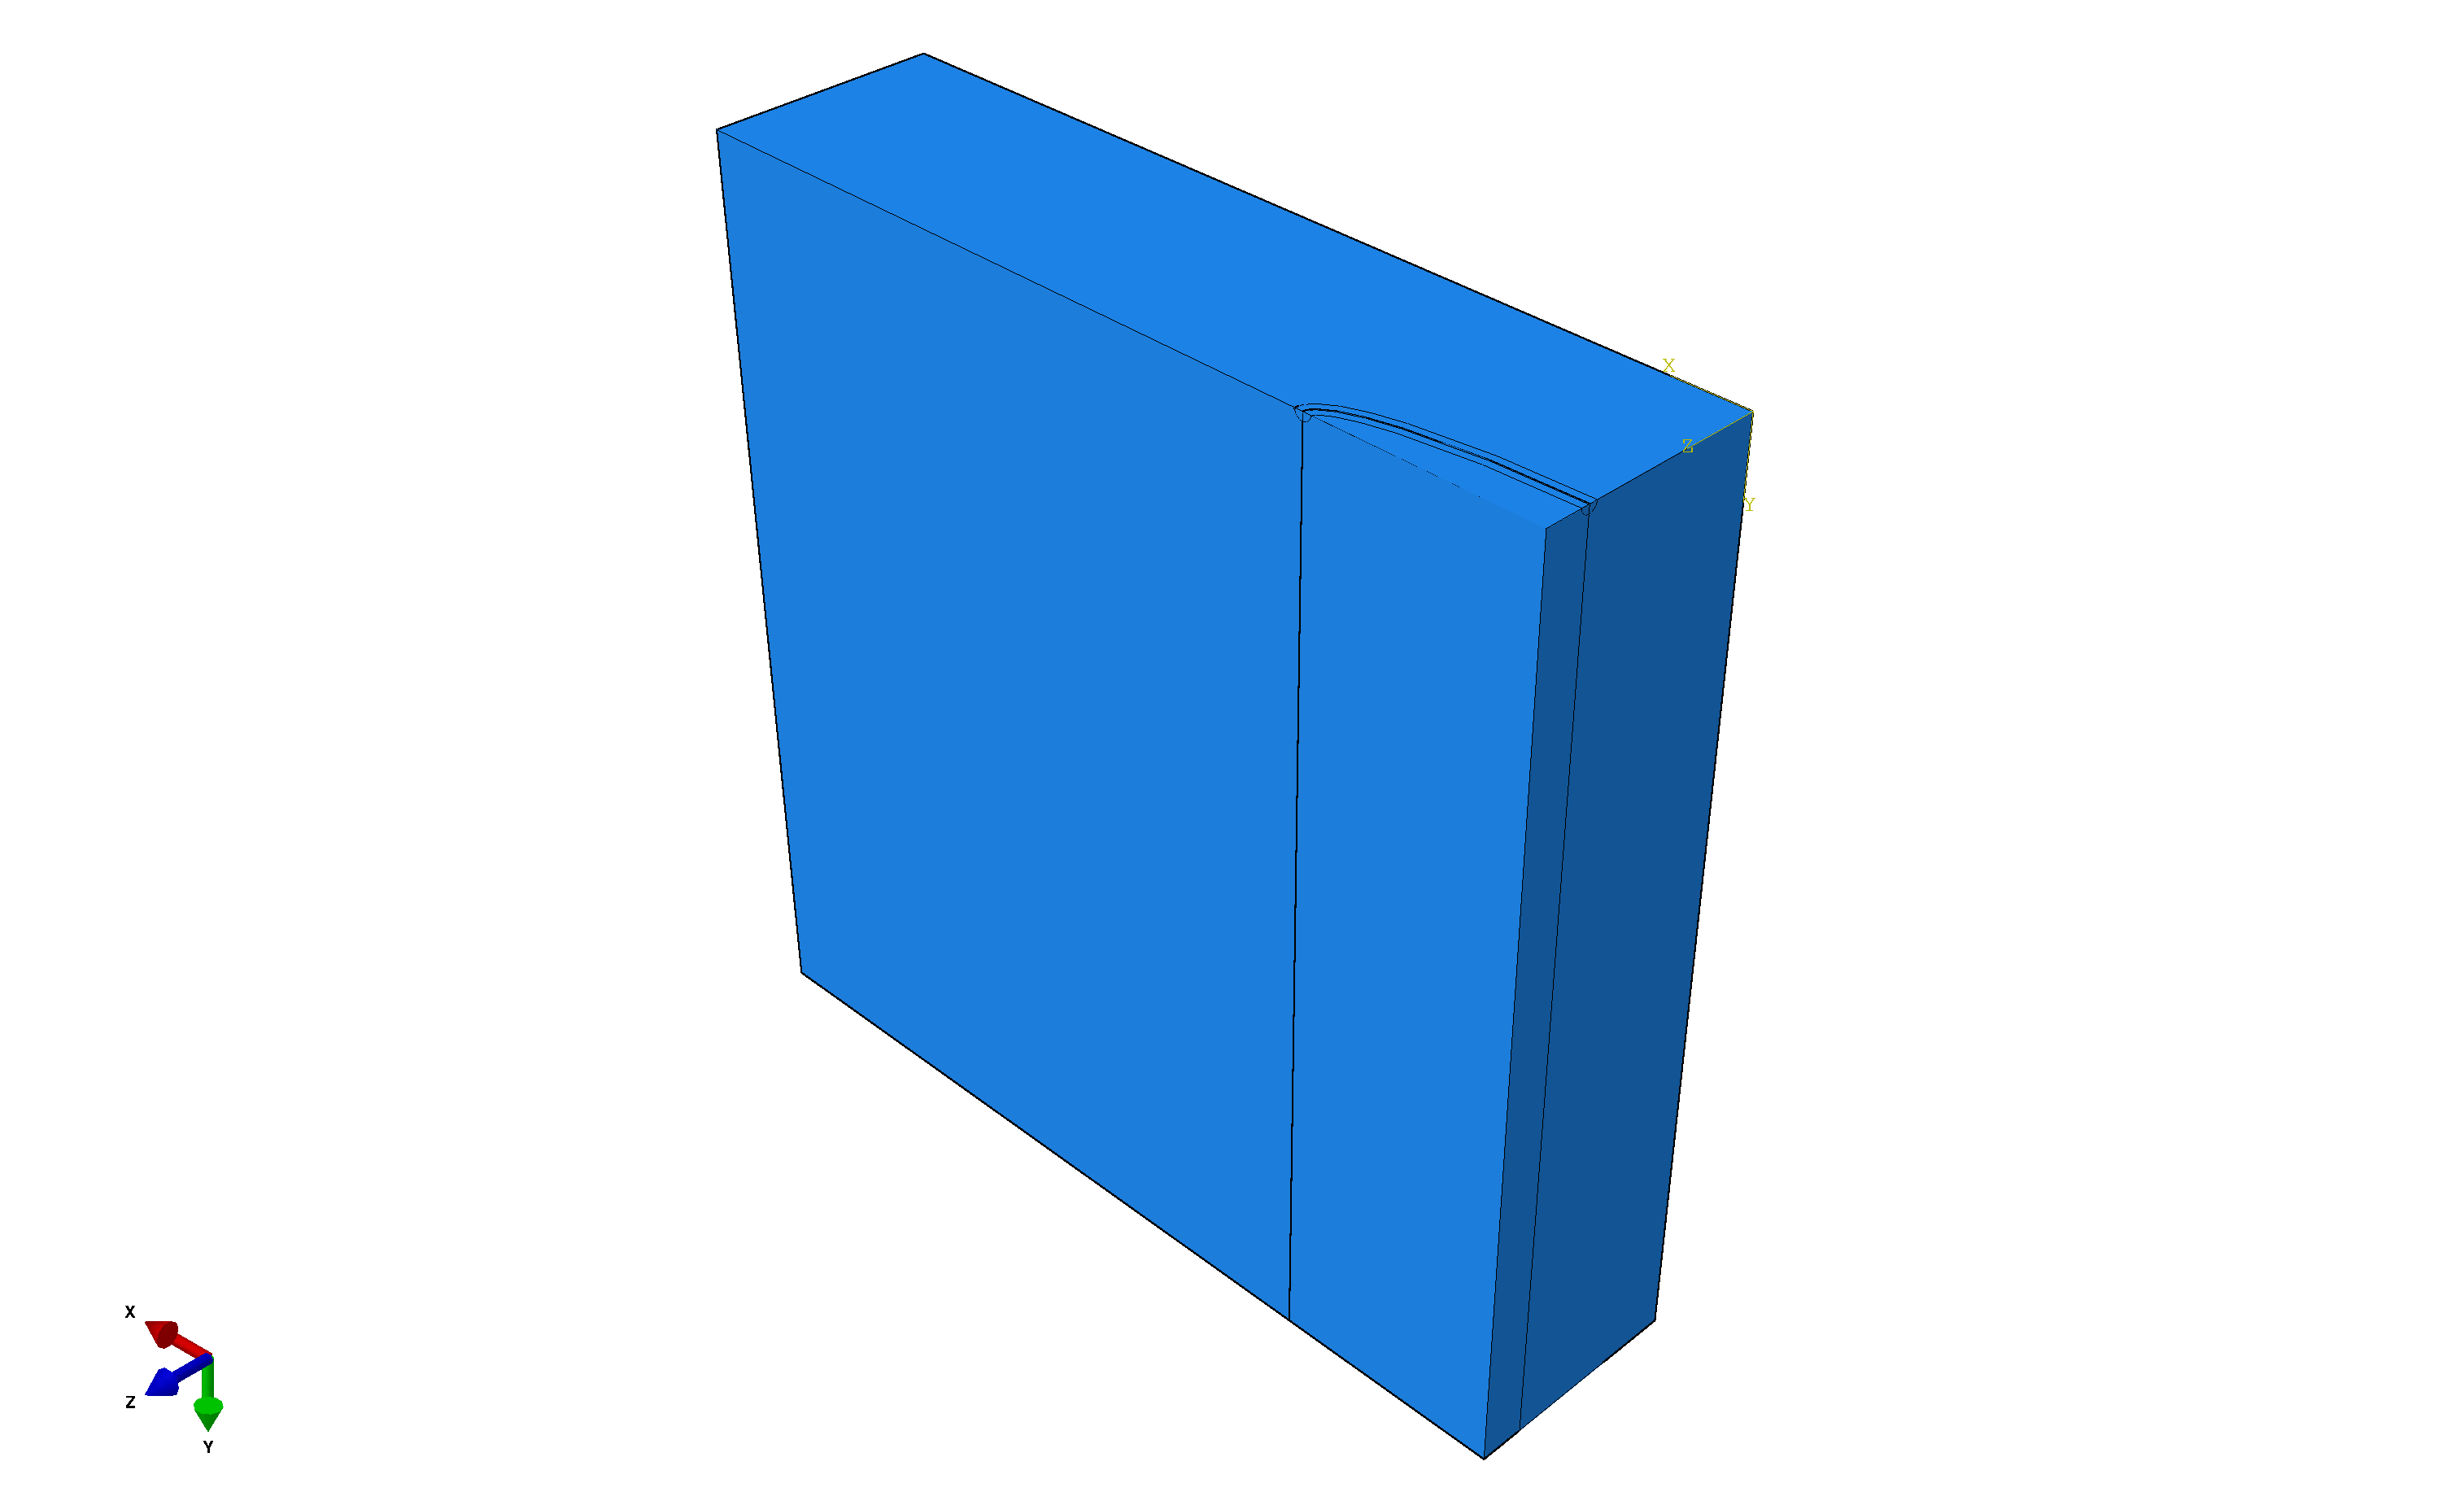
\includegraphics[width=\columnwidth]{model1-assembly}
    \caption{McClung et al. model 1\label{fig:model1-assembly}}
  \end{figure}
  \begin{figure}
    \centering
    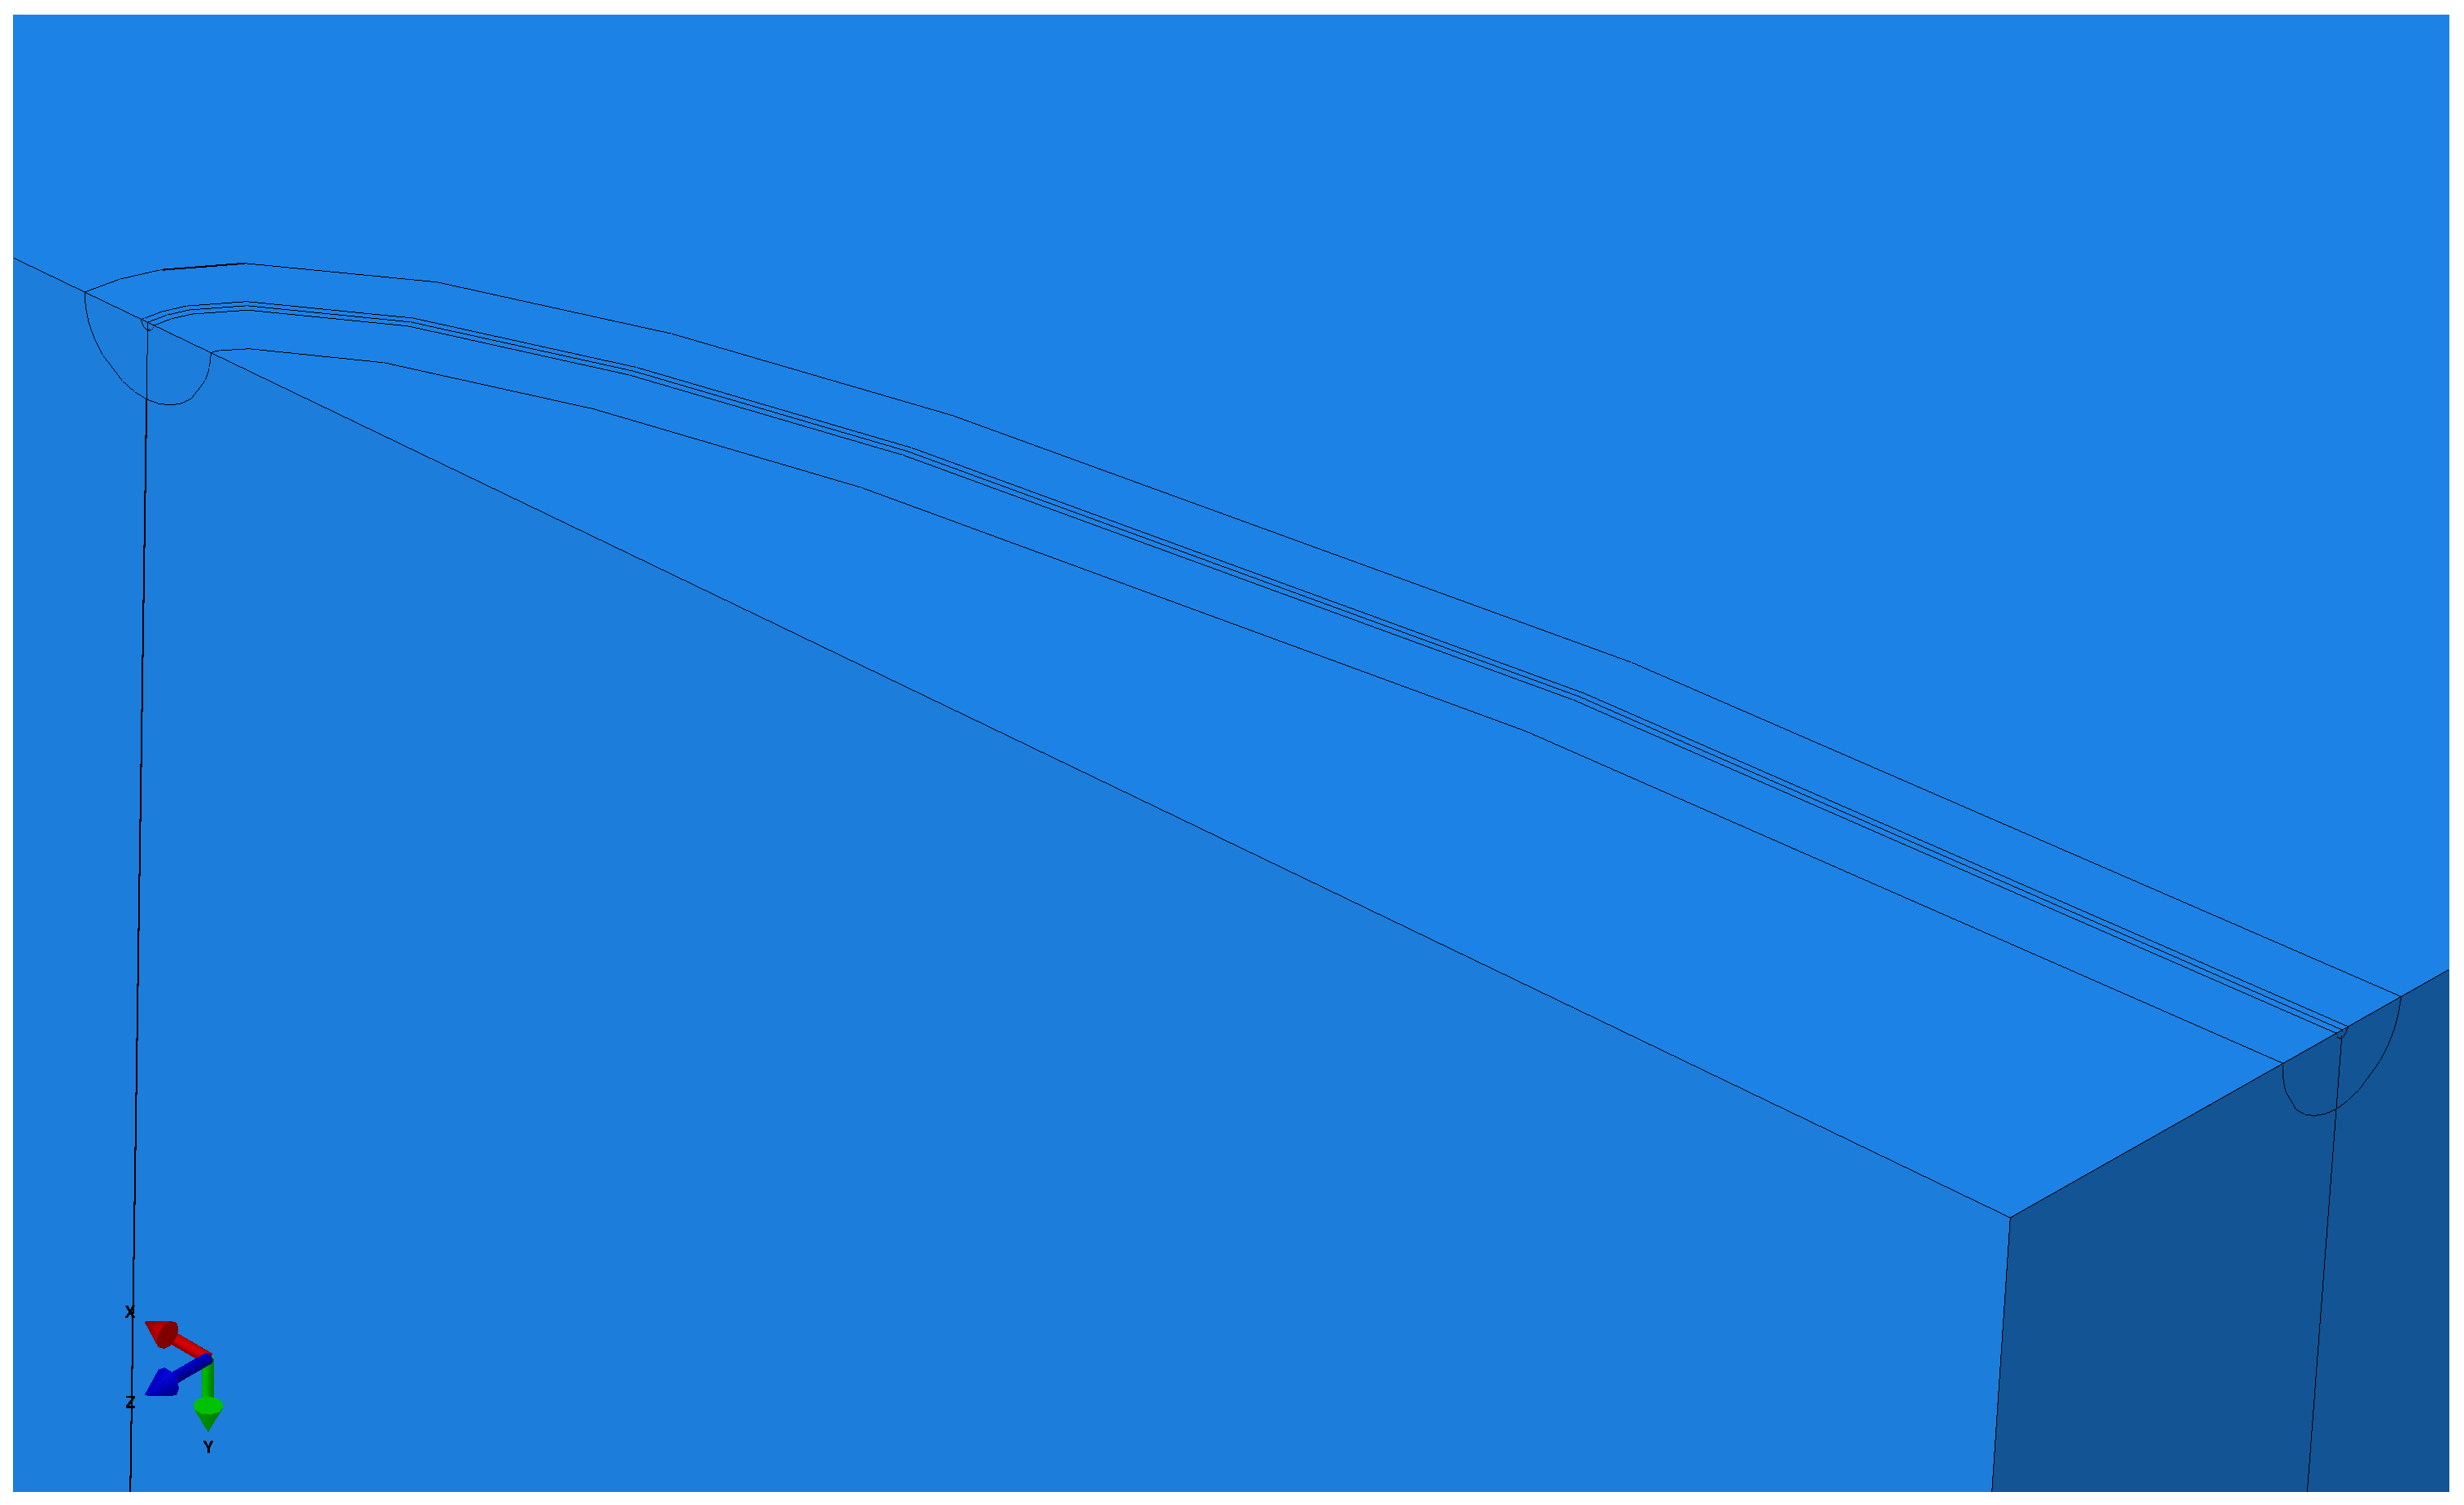
\includegraphics[width=\columnwidth]{model1-assembly-zoomed}
    \caption{McClung et al. model 1 crack front detail\label{fig:model1-assembly-zoomed}}
  \end{figure}
  \begin{figure}
    \centering
    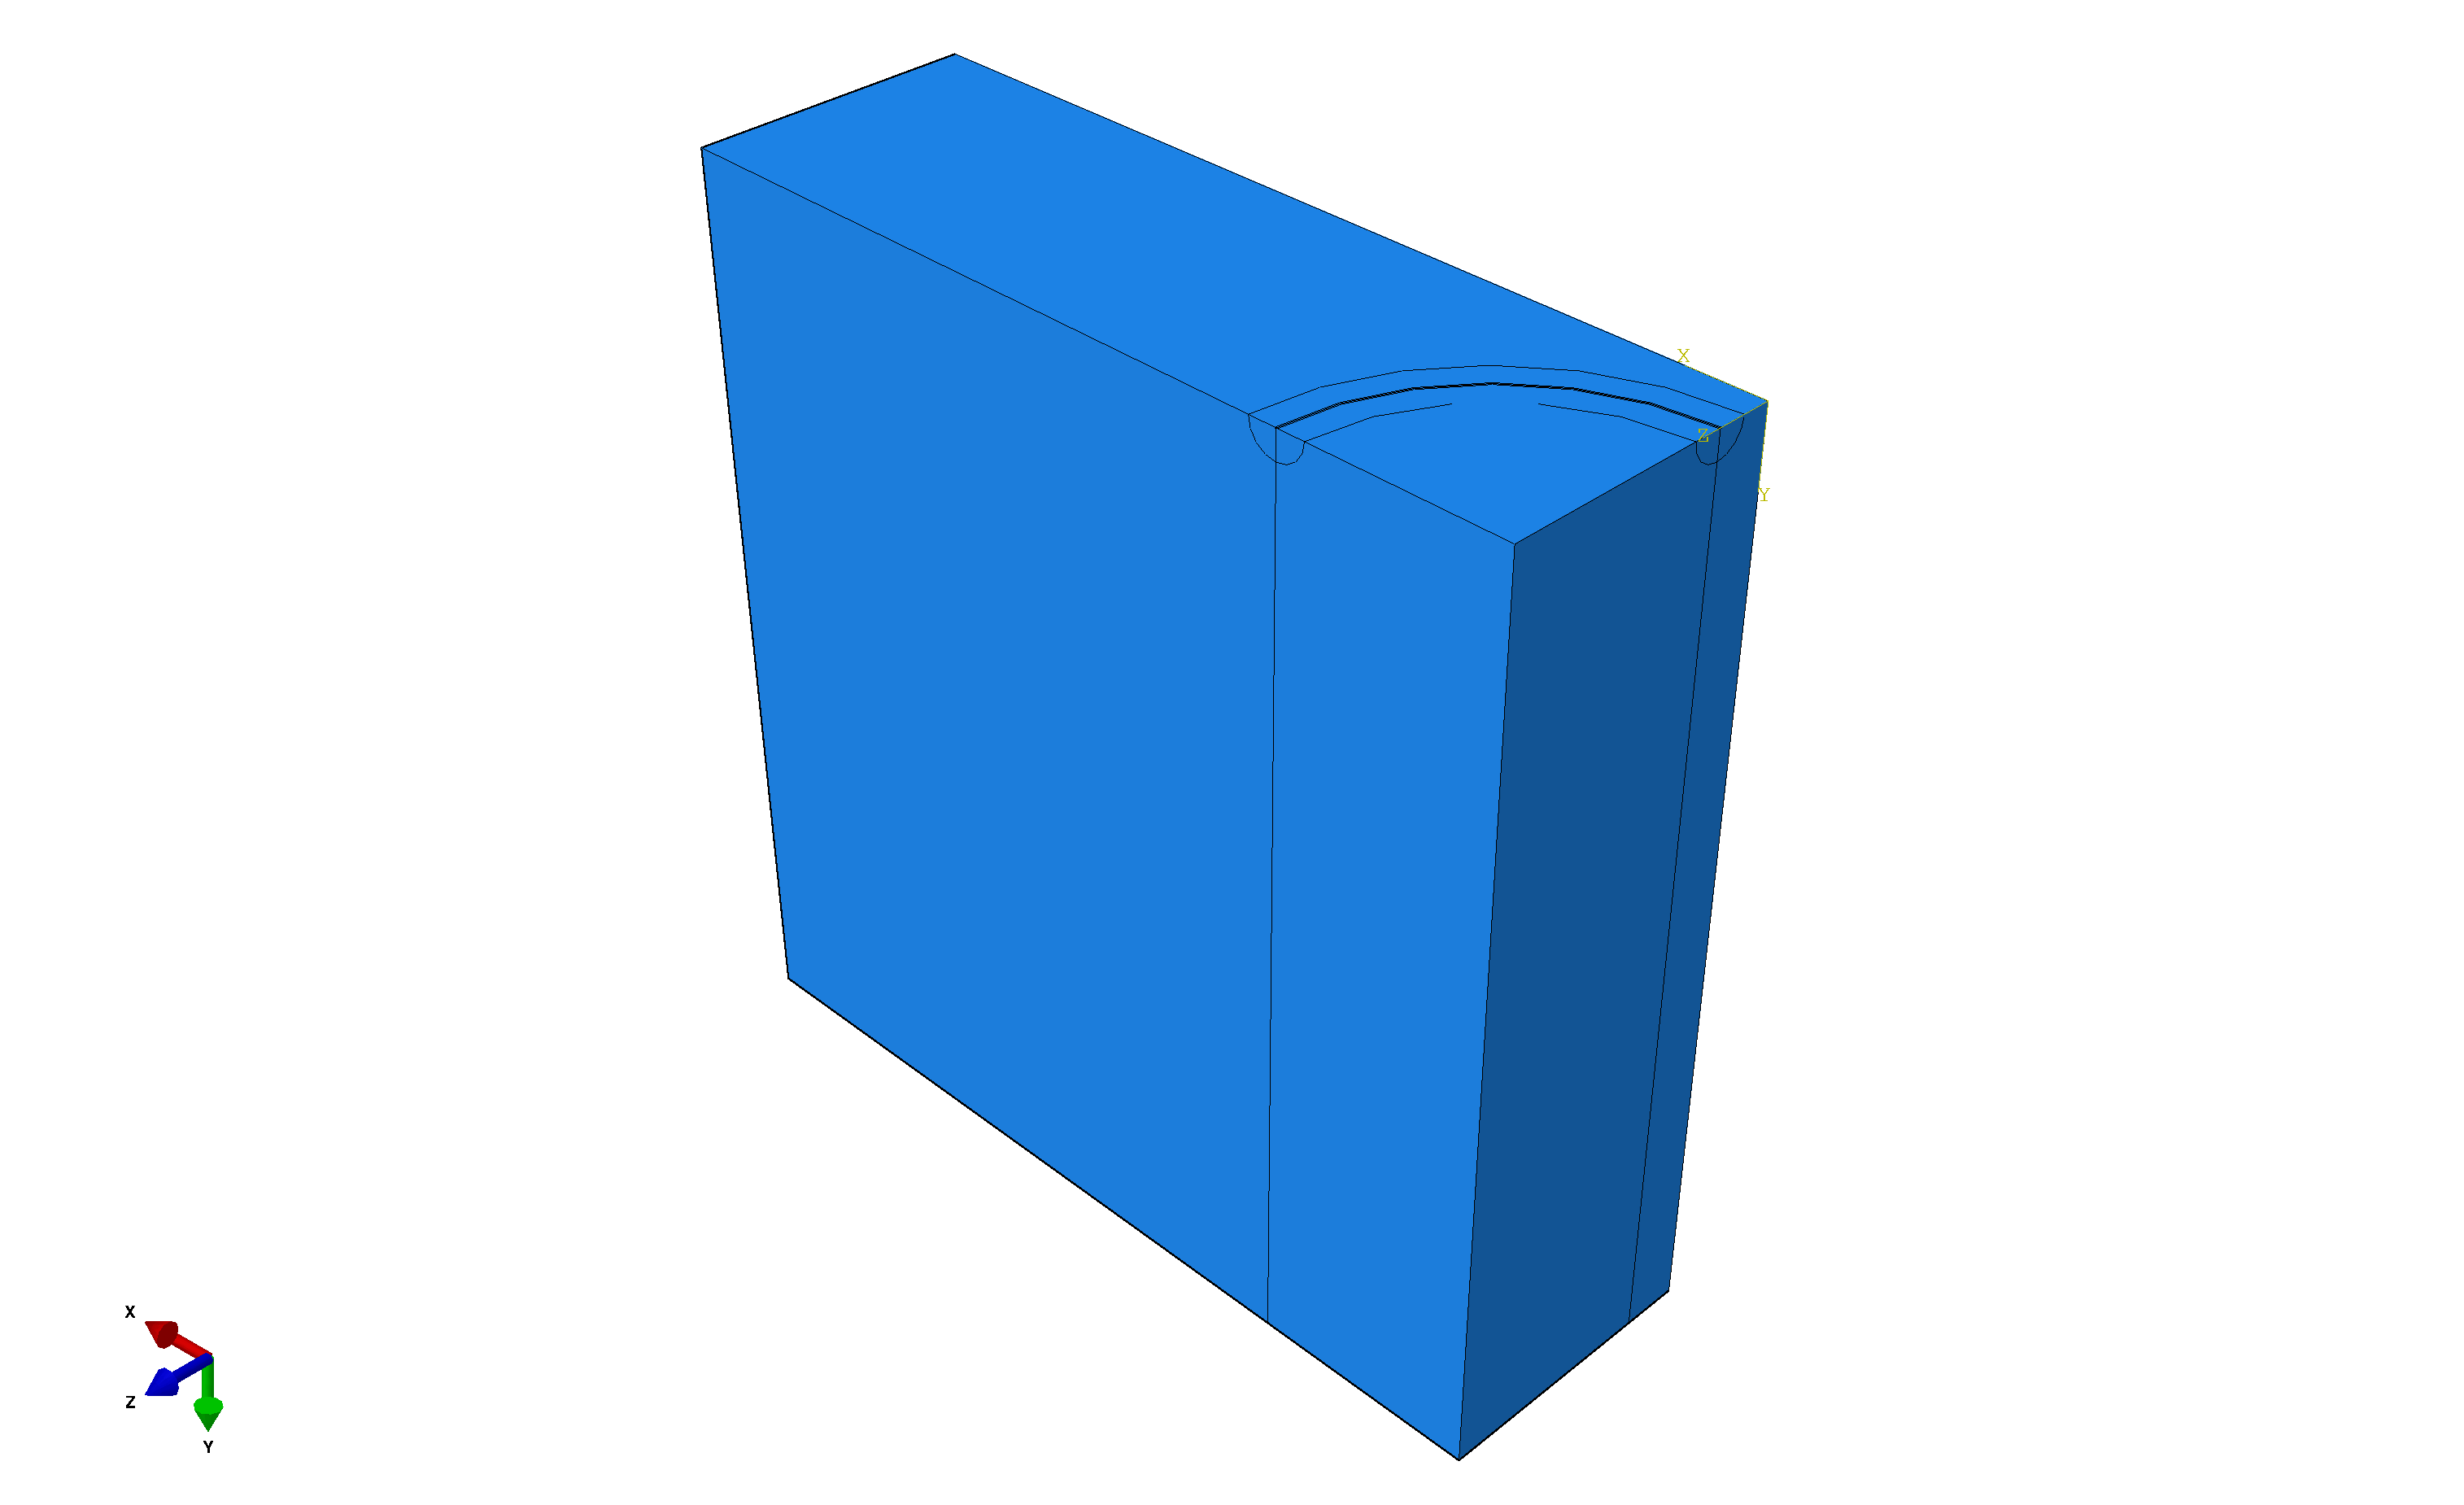
\includegraphics[width=\columnwidth]{model9-assembly}
    \caption{McClung et al. model 9\label{fig:model9-assembly}}
  \end{figure}
